\documentclass[a4paper,12pt]{article}
%%%%%%%%%%%%%%%%%%%%%%%%%%%%%%%%%%%%%%%%%%%%%%%%%%%%%%%%%%%%%%%%%%%%%%%%%%%%%%%%%%%%%%%%%%%%%%%%%%%%%%%%%%%%%%%%%%%%%%%%%%%%%%%%%%%%%%%%%%%%%%%%%%%%%%%%%%%%%%%%%%%%%%%%%%%%%%%%%%%%%%%%%%%%%%%%%%%%%%%%%%%%%%%%%%%%%%%%%%%%%%%%%%%%%%%%%%%%%%%%%%%%%%%%%%%%
\usepackage{eurosym}
\usepackage{vmargin}
\usepackage{amsmath}
\usepackage{graphics}
\usepackage{epsfig}
\usepackage{enumerate}
\usepackage{multicol}
\usepackage{subfigure}
\usepackage{fancyhdr}
\usepackage{listings}
\usepackage{framed}
\usepackage{graphicx}
\usepackage{amsmath}
\usepackage{chngpage}
%\usepackage{bigints}

\usepackage{vmargin}
% left top textwidth textheight headheight
% headsep footheight footskip
\setmargins{2.0cm}{2.5cm}{16 cm}{22cm}{0.5cm}{0cm}{1cm}{1cm}
\renewcommand{\baselinestretch}{1.3}

\setcounter{MaxMatrixCols}{10}

\begin{document}
\Large 

\begin{itemize}
    \item Use the command \texttt{set.seed(2019)} to initialise the random number generator.

    \item When you execute any R code, make sure you run the entire R script including the line \texttt{set.seed(2019)} .
\end{itemize}
\begin{framed}\begin{verbatim}
sample(1:6,10,replace=TRUE)

set.seed(2019)
sample(1:6,10,replace=TRUE)
\end{verbatim}\end{framed}
\newpage 
\begin{center}
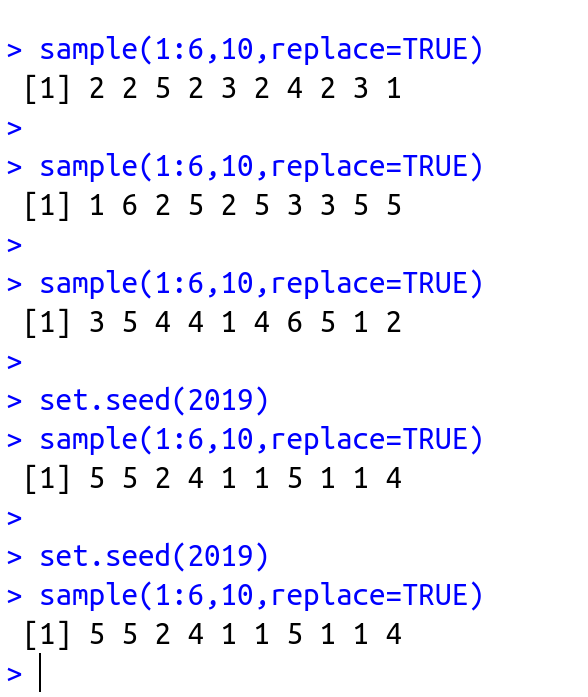
\includegraphics[scale=0.5]{00-C1/images/00-C1-Q3-Setseed.png}    
\end{center}


\newpage 

\subsection*{Exercise 1}

\noindent Consider a random sample $X_1 , \ldots , X_n$ from an Exponential distribution with parameter $\lambda$ and define 
$$ Y = \sum^{n}_{i=1} X_i $$

\noindent State the distribution of $Y$, giving all the parameters of the distribution.


%%%%%%%%%%%%%%%%%%%%%%
\begin{framed}
\large 
\noindent Theory
\begin{itemize}
    \item The sum of $n$ exponential ($\lambda$) random variables is a gamma ($n, \lambda$) random variable.
    \item The rate parameter is usually denoted as $\beta$ for the Gamma Distribution, i.e. gamma ($n, \beta$) 

 \item Mean for Gamma Distribution	 ${\displaystyle {\frac {\alpha }{\beta }}} $

\item Variance	for Gamma Distribution $ {\displaystyle {\frac {\alpha }{\beta ^{2}}}}$

    \item If the exponential random variables have a common rate parameter, their sum has an Erlang distribution, a special case of the gamma distribution.
\end{itemize}
\end{framed}

\noindent The distribution of $Y$ is a Gamma distribution,
$$Y \sim \mbox{Gamma}(n, \lambda)$$
%%%%%%%%%%%%%%%%%%%%%%%%%%%%%%%%%%%
\newpage 

\begin{framed}
\begin{verbatim}
set.seed(2019);rexp(5,0.5)

set.seed(2019);sum(rexp(5,0.5))

set.seed(2019)
X = replicate(1000,sum(rexp(20,0.5)))

mean(X)

var(X)

\end{verbatim}
\end{framed}

\newpage 
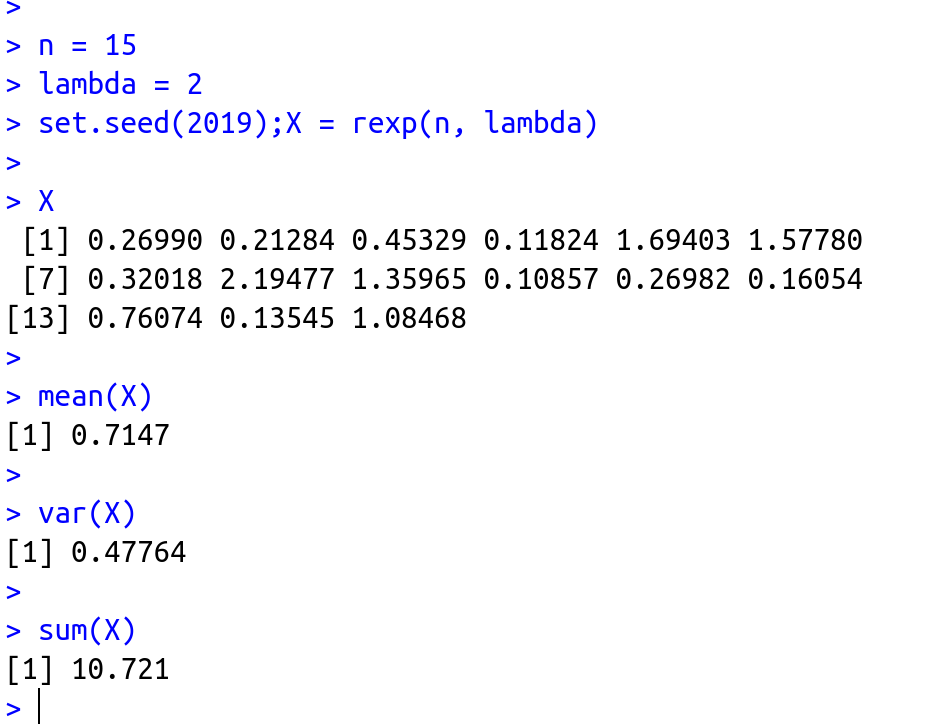
\includegraphics[scale=0.5]{00-C1/images/00-C1-Q3-2.png}
\newpage 
\subsection*{Exercise 2}

Perform simulation of a sample $x_1 , ..., x_n$ with sample size n = 15 from an
exponential distribution with parameter $\lambda = 2$.


\begin{framed}\begin{verbatim}
n = 15
lambda = 2
set.seed(2019);X = rexp(n, lambda)

X 

mean(X)

var(X)

sum(X) 


\end{verbatim}\end{framed}





\newpage 

\subsection*{Exercise 3}

Calculate the value of Y for the sample in part 2.

\begin{framed}\begin{verbatim}
Y = sum(X)
\end{verbatim}\end{framed}



\newpage 
\subsection*{Exercise 4}
\noindent Perform 1,000 repetitions of parts 2 and 3 to obtain a Bootstrap sample
$y_1 , ..., y_B$ from the random variable Y with B = 1,000.


\noindent Using \texttt{for} loops.
\begin{framed}\begin{verbatim}
y = 0*(1:1000) # generate a vector of size 1000

for (i in 1:1000){

   y[i] = sum(rexp(n, lambda))

} 
\end{verbatim}\end{framed}

\noindent Using \texttt{replicate()}
\begin{framed}\begin{verbatim}

y = replicate(1000, sum(rexp(n, lambda)))

\end{verbatim}\end{framed}
%%%%%%%%%%%%%%%%%%%%%%%%%%%%%%%%%%%%%%%%%%%%%%%%%%%%%%%%%%%
\newpage 
\subsection*{Exercise  5}

Plot a histogram showing the relative frequencies of the sample $y_1 , ..., y_B$  from
part 4.

\begin{framed}\begin{verbatim}
hist(y, prob=TRUE) 
\end{verbatim}\end{framed}


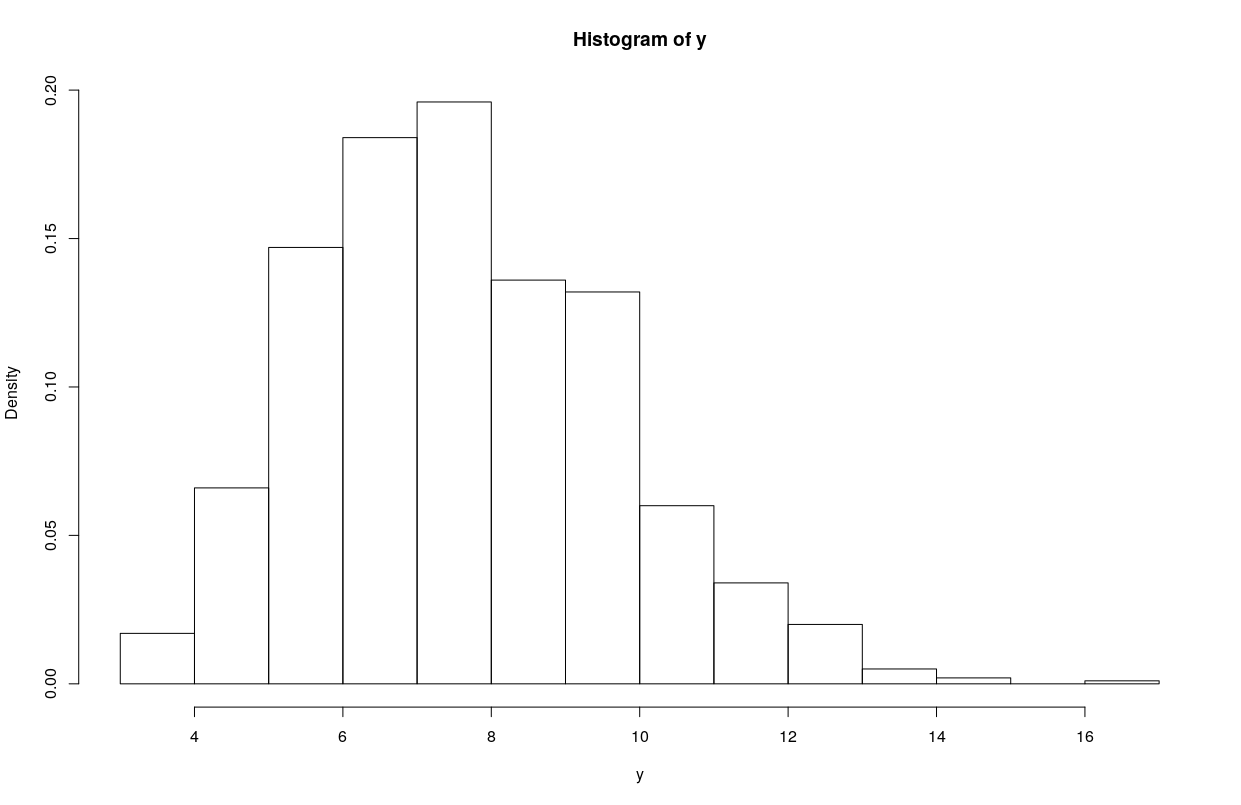
\includegraphics[scale=0.55]{00-C1/images/00-C1-Q3-Hist.png}
%%%%%%%%%%%%%%%%%%%%%%%%%%%%%%%%%%%%%%%%%%%%%%%%%%%%%5
\newpage

\subsection*{Exercise 6}
\noindent Compare graphically the histogram in part 4 to the density of a
suitable Normal distribution. You might find the following R command
useful:

\begin{framed}\begin{verbatim}
curve(dnorm(x,mean= ...., sd= ... , 
    add=TRUE, 
    lwd=2,
    col="red"))
\end{verbatim}\end{framed}


\begin{framed}\begin{verbatim}
hist(y,prob=TRUE,
     xlim=c(0,20),
     ylim=c(0,0.25))

curve(dnorm(x,
            mean=n/lambda,
            sd=sqrt(n/(lambda^2))), 
      add=TRUE, lwd=2, col="red")

\end{verbatim}\end{framed}

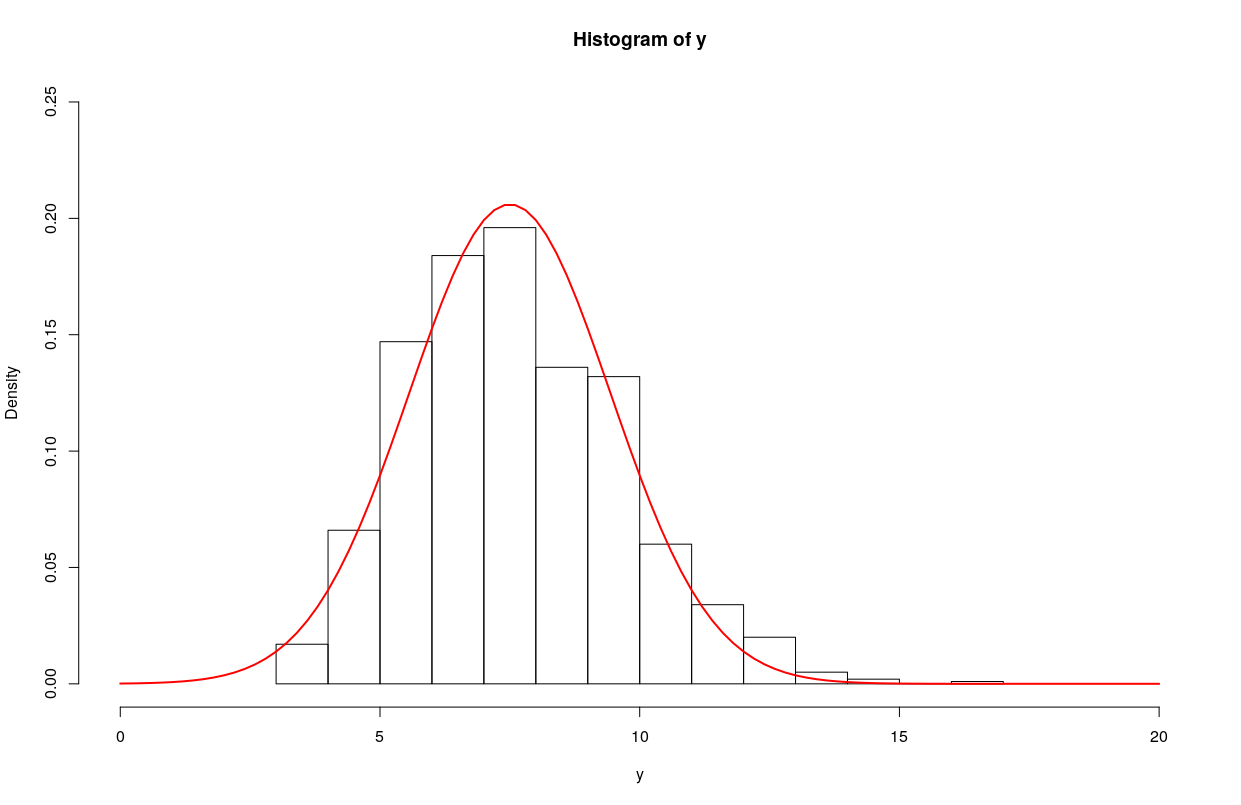
\includegraphics[scale=0.6]{00-C1/images/00-C1-Q3-Curve.png}

\newpage

\begin{framed}\begin{verbatim}
hist(y,prob=TRUE,
     xlim=c(0,20),
     ylim=c(0,0.225),
     col=c("pink","lightblue"))

curve(dnorm(x,
            mean=n/lambda,
            sd=sqrt(n/(lambda^2))), 
      add=TRUE, lwd=2.75, 
      col="red")


\end{verbatim}\end{framed}

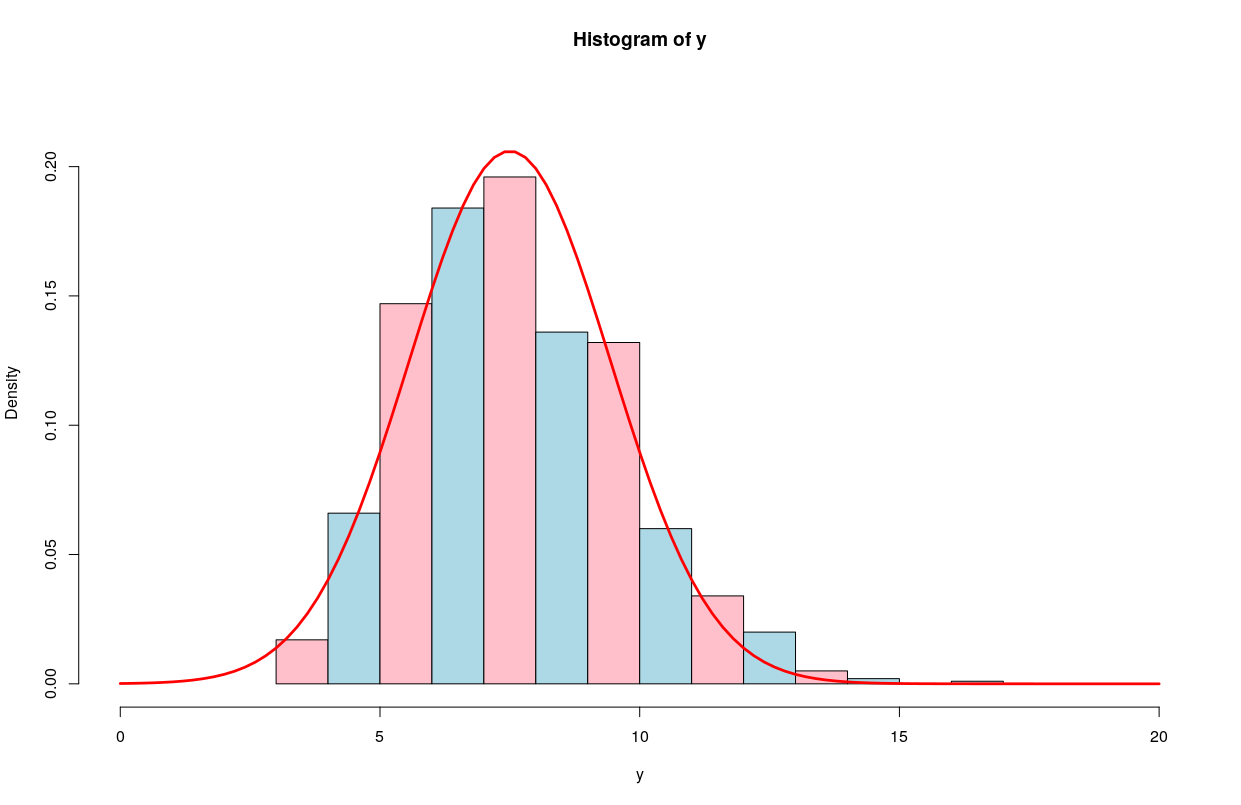
\includegraphics[scale=0.6]{00-C1/images/00-C1-Q3-Curve-2.png}


%%%%%%%%%%%%%%%%%%%%%%%%%%%%%%555
\newpage 

\noindent Comment on your findings in the context of the Central
Limit Theorem.

\begin{itemize}
    \item In contrast to a normal distribution, the histogram is clearly not symmetrical.

\item This comes from the fact that $Y$ can take only positive values.
For a larger sample size of $n$ of $x_1 , ... , x_n$ (not a larger B) the CLT ensures that the
distribution of $Y$ becomes approximately normal.
\end{itemize}

\newpage
\begin{framed}
\begin{verbatim}
n = 75
lambda = 2
set.seed(2019)
y = replicate(1000, sum(rexp(n, lambda)))

hist(y,prob=TRUE,
     xlim=c(20,60),
     ylim=c(0,0.10),
     col=c("pink","lightblue"))

curve(dnorm(x,
            mean=n/lambda,
            sd=sqrt(n/(lambda^2))), 
      add=TRUE, lwd=2.75, 
      col="red")

\end{verbatim}
\end{framed}
\newpage
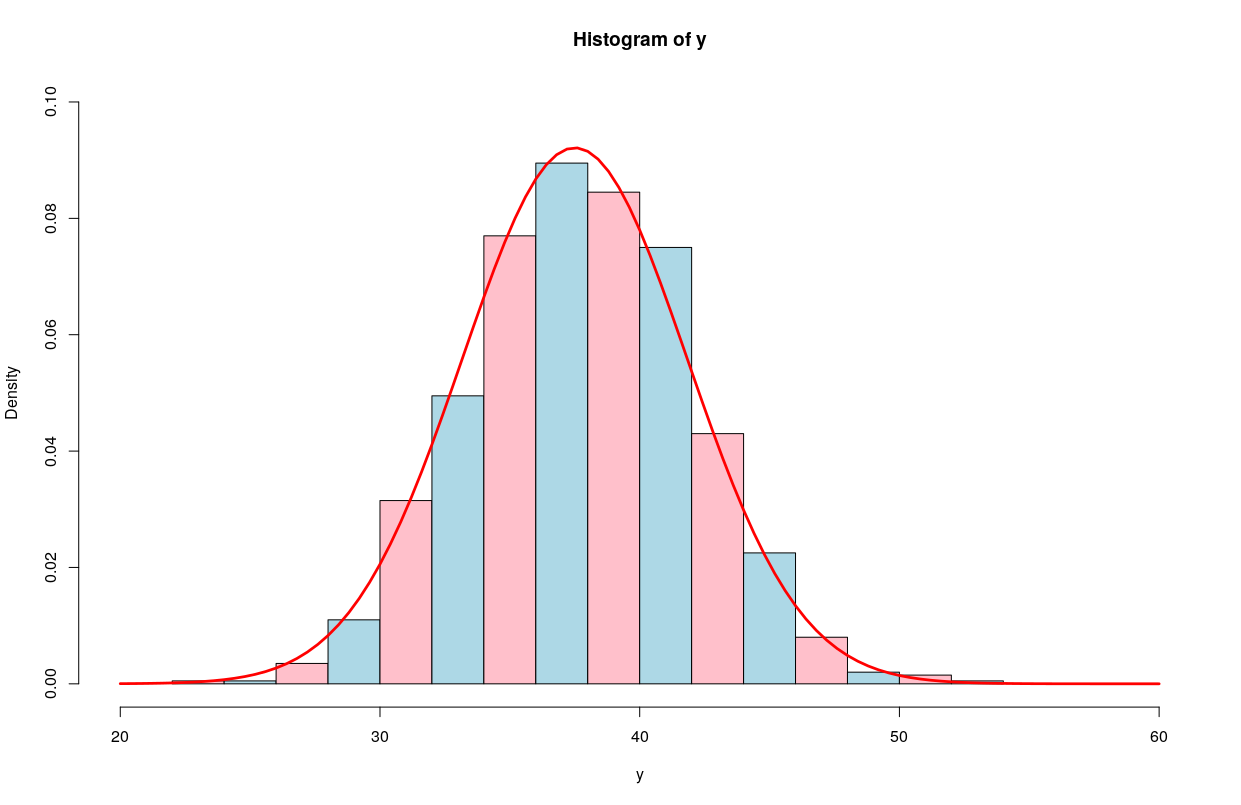
\includegraphics[scale=0.5]{00-C1/images/00-C1-Q3-Curve-Q3.png}

%%%%%%%%%%%%%%%%%%%%%%%%%%%%%%555
\newpage 
Parts (i)-(iii) were generally very well answered. In part (iv) there was wide variation in
the quality of the answers with various errors in the details of the code. 

A common error in part (v) was omitting the (prob = TRUE) part of the code, which is required for relative frequencies. 

Part (vi)(a) was reasonably well attempted, while many candidates did not
attempt part (vi)(b), with some giving incomplete comments. Part (vi)(a) can alternatively
be answered using R code based on the lines() command.


\end{document}
